\section{Results}

\subsection{Best accepted model}

The best accepted model is \texttt{timed\_s0\_d40\_m170\_f0p35\_e1p00}. It starts at 0 Myr, lasts 40 Myr, uses representative $170\,M_\odot$ PopIII/PISN-like yields, has fraction 0.35, and assumes full mixing efficiency.

It reaches code-light \simg=0.372 and E-MILES NIR-local \simg=0.499. Its relic-fit deltas are $\Delta\mh=+0.095$, $\Delta\mgfe=-0.070$, $\Delta\log M=+0.137$, and $\Delta\log M/L=+0.053$. This is final-enough for discussion and lies within the adopted relic-fit tolerance box, but it is a boundary solution.

\begin{figure}
\centering
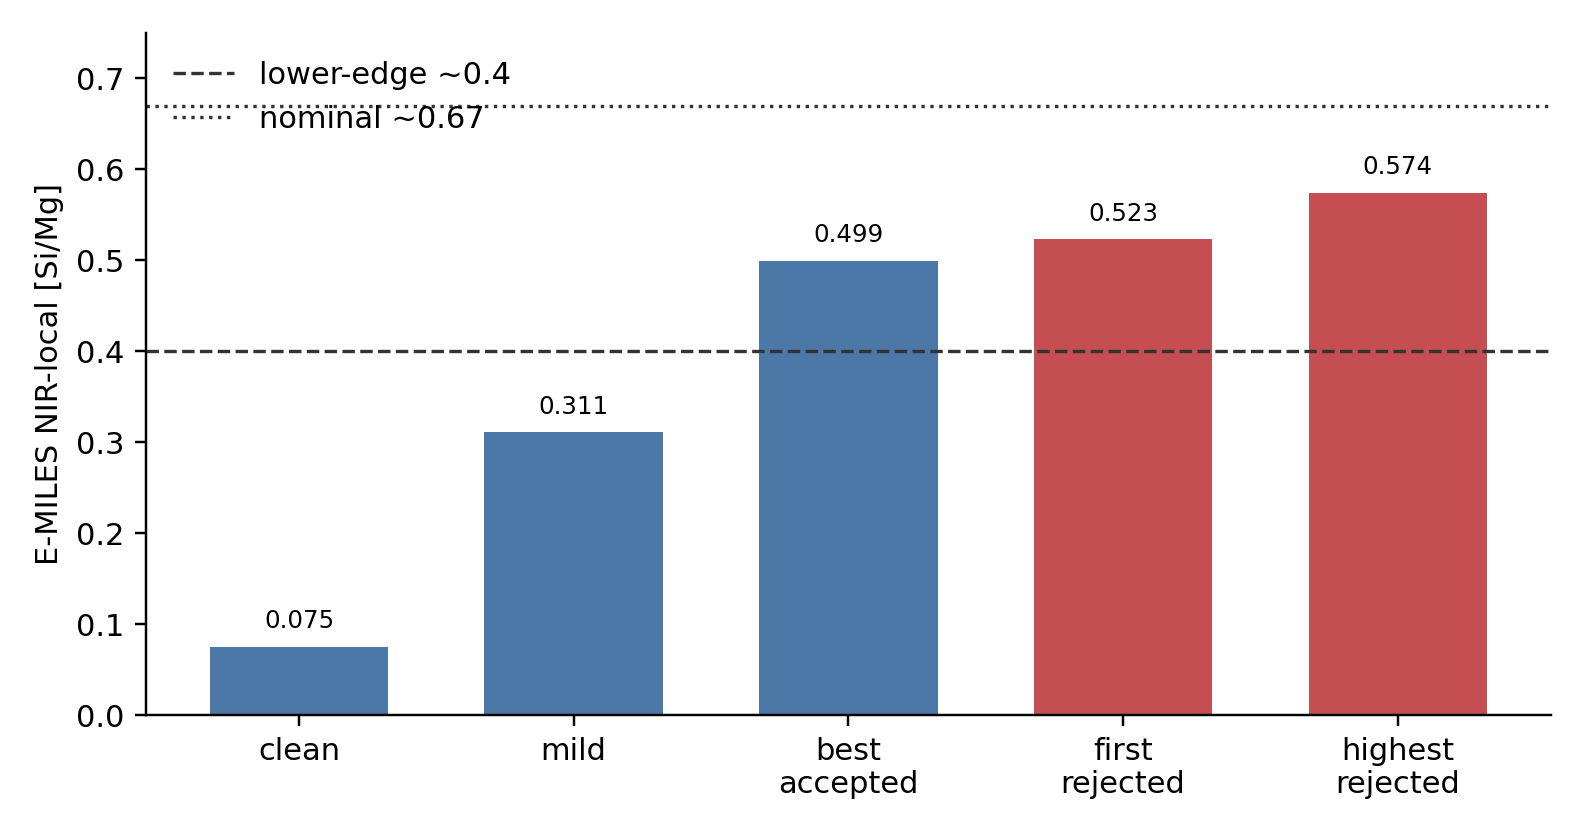
\includegraphics[width=\columnwidth]{figures/final_relic_simg_key_models.png}
\caption{Current key model comparison from the lightweight analysis products. The clean baseline stays at low \simg, while the best accepted timed Si-rich enrichment model reaches the lower high-Si regime. This figure should be remade in final A\&A style before submission.}
\label{fig:key_models}
\end{figure}

\subsection{First rejected higher-Si/Mg model}

The matched 50 Myr counterpart, \texttt{timed\_s0\_d50\_m170\_f0p35\_e1p00}, reaches E-MILES NIR-local $\simg\simeq0.523$, but is rejected. Its deltas are $\Delta\mh=+0.113$, $\Delta\mgfe=-0.085$, $\Delta\log M=+0.168$, and $\Delta\log M/L=+0.072$. The failures are total metallicity, \mgfe, and stellar mass; $M/L$ is less restrictive.

\subsection{Failure modes}

The high-Si failure modes are coupled. Raising Si/Mg by increasing or extending the mixed channel changes the integrated metal budget, depresses \mgfe, and shifts stellar mass. A successful enrichment channel must be Si-selective, localized, short-lived, or spectrally/aperture-weighted in a way that affects the NIR indices more than the whole one-zone relic.

% TODO figure placeholder:
% \begin{figure}
% \centering
% \includegraphics[width=\columnwidth]{figures/simg_pareto_failure_modes.pdf}
% \caption{Planned Si/Mg versus relic-fit degradation plot. Source tables: constrained_simg_local_refinement_v1.csv and high_simg_failure_modes_v1.csv.}
% \label{fig:pareto}
% \end{figure}

\subsection{Why NIR weighting alone is insufficient}

E-MILES NIR-local weighting increases the clean baseline by only 0.018 dex, from \simg=0.058 to about 0.075. It helps only when a chemically Si-rich population already exists. Therefore, weighting alone does not explain the baseline discrepancy.

% TODO figure placeholder:
% \begin{figure}
% \centering
% \includegraphics[width=\columnwidth]{figures/emiles_nir_weighting_effect.pdf}
% \caption{Planned comparison of current code-light and E-MILES NIR-local \simg\ values. Source table: emiles_nir_flux_weighted_abundances_v1.csv.}
% \label{fig:emiles_weighting}
% \end{figure}

\subsection{Normal ETG control sequence}

The NGC~1277 experiment needs a control population: normal early-type galaxies should not preserve the same strong Si-rich signature as a compact relic. We therefore compare the relic-strength channel with a weak/moderate fixed diagnostic sequence for ETG models calibrated to the mass--metallicity and mass--\mgfe\ relations. These tests are copied-code fixed diagnostics, not new optimizations. M1e9, M1e10, and M1e11 use current total-mass ETG rows as upper-limit controls, while M1e12 uses the validated $f_{\rm core}=0.8$ core model.

\begin{table*}
\caption{Weak/moderate PopIII/PISN-like Si-rich control sequence for fixed ETG diagnostics.}
\label{tab:weakmod_etg_sequence}
\centering
\begin{tabular}{lccccc}
\toprule
Mass & Clean & 20 Myr, $f=0.10$ & 40 Myr, $f=0.10$ & 20 Myr, $f=0.20$ & 40 Myr, $f=0.20$ \\
\midrule
M1e9  & 0.192 & 0.246 & 0.277 & 0.293 & 0.347 \\
M1e10 & 0.147 & 0.178 & 0.197 & 0.207 & 0.242 \\
M1e11 & 0.093 & 0.113 & 0.126 & 0.132 & 0.155 \\
M1e12 & 0.074 & 0.129 & 0.160 & 0.175 & 0.229 \\
\bottomrule
\end{tabular}
\tablefoot{Entries are chemical-evolution abundance proxies for \simg. M1e9 is treated as a low-mass upper-limit diagnostic rather than a normal massive ETG anchor. The M1e12 row uses the validated $f_{\rm core}=0.8$ core model; the lower-mass rows use existing total-mass fixed ETG diagnostics.}
\end{table*}


\begin{figure}
\centering
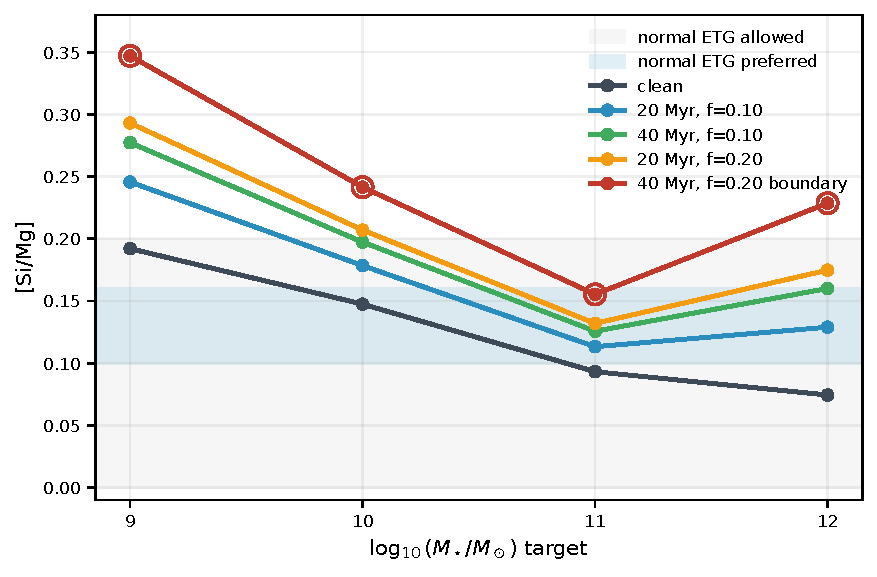
\includegraphics[width=\columnwidth]{figures/weakmod_etg_simg_sequence.pdf}
\caption{Weak/moderate Si-rich fixed diagnostic sequence for ETG controls. The conservative normal-ETG channel is the 20 Myr, $f=0.10$ case. M1e9 starts close to the upper normal \simg\ range and is therefore treated as a low-mass upper-limit diagnostic.}
\label{fig:weakmod_sequence}
\end{figure}

\begin{figure}
\centering
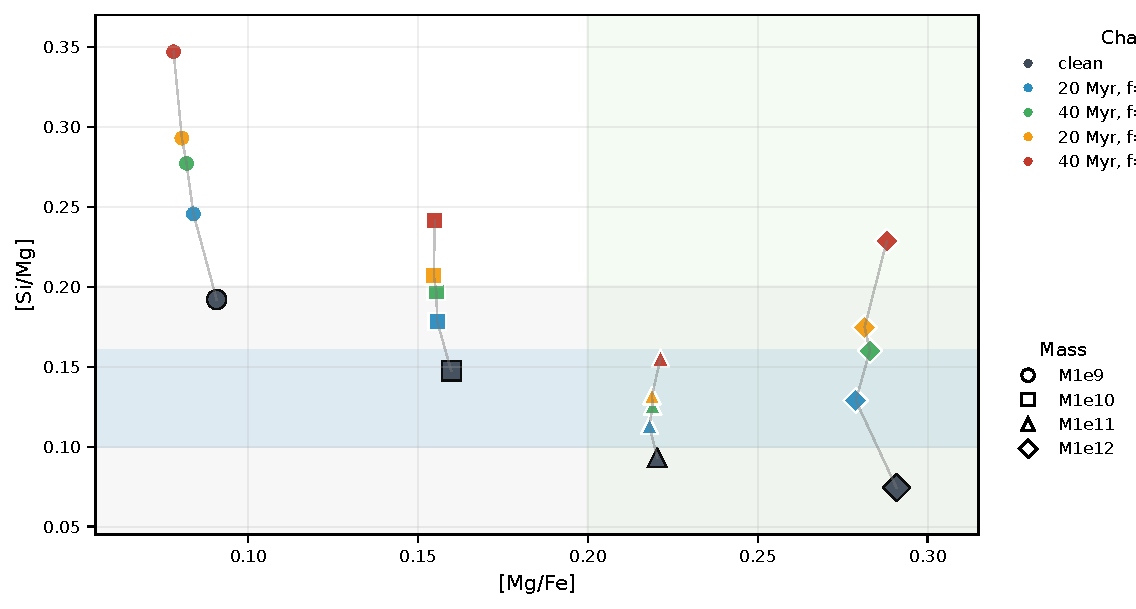
\includegraphics[width=\columnwidth]{figures/weakmod_etg_simg_vs_mgfe.pdf}
\caption{Control-sequence \simg\ versus \mgfe. The models preserve the calibration role of \mgfe\ while \simg\ separates the strength of preserved early Si-rich enrichment.}
\label{fig:weakmod_simg_mgfe}
\end{figure}

The safest normal-ETG preserved Si-rich channel is the 20 Myr, $f=0.10$ case. It remains compatible for M1e10, M1e11, and M1e12 while modifying \simg\ without breaking the stored mass, metallicity, and \mgfe\ calibration. The 40 Myr, $f=0.20$ case is best treated as an upper-normal or boundary case. The relic-strength $f=0.35$ channel is therefore reserved for NGC~1277-like high-preservation systems rather than normal ETG calibration.

\begin{figure}
\centering
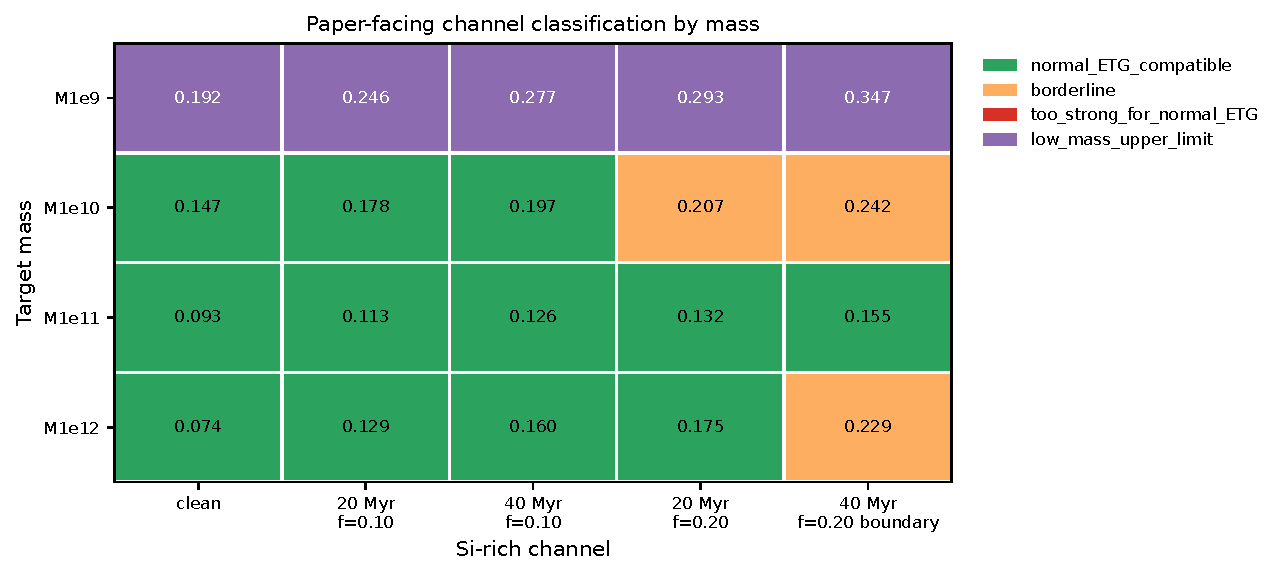
\includegraphics[width=\columnwidth]{figures/weakmod_allowed_channel_strength_by_mass.pdf}
\caption{Paper-facing classification of weak/moderate Si-rich channels by mass. The classification uses the multi-constraint calibration: stellar mass, metallicity, \mgfe, and whether \simg\ is in or can be diluted into the normal ETG locus with an old alpha-enhanced envelope.}
\label{fig:weakmod_allowed_strength}
\end{figure}

\begin{figure}
\centering
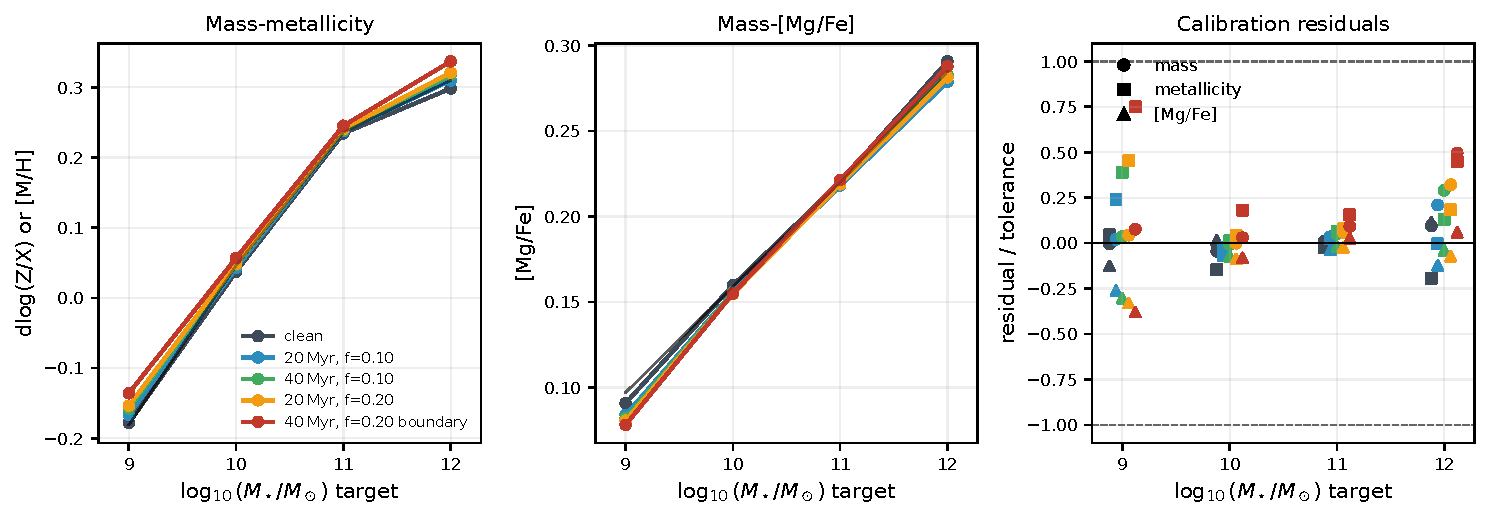
\includegraphics[width=\columnwidth]{figures/weakmod_mass_metallicity_mgfe_validation.pdf}
\caption{Mass--metallicity and mass--\mgfe\ validation for the weak/moderate control sequence. Accepted channels preserve the global ETG calibration while changing \simg.}
\label{fig:weakmod_validation}
\end{figure}
